\documentclass[../main.tex]{subfiles}
\graphicspath{{\subfix{../figures/}}}

\begin{document}
\section{UML中的用例图}
\textbf{用例模型}:用例模型描述的是用户所理解的系统功能。用例驱动的系统分析与设计方法,已成为面向对象系统分析与设计的主流方法。
\begin{itemize}
  \item 它描述了待开发系统的\textbf{功能需求};
  \item 它将系统看作\textbf{黑盒},从外部执行者的角度来理解系统;
  \item 它\textbf{驱动}了需求分析之后各阶段的开发工作,不仅在开发过程中保证了系统所有功能的实现,而且被用于验证和检测所开发的系统,从而影响到开发工作的各个阶段和 UML 的各个模型。
\end{itemize}
在UML中,一个用例模型由若干个用例图描述,用例图主要元素是用例和执行者。
\begin{figure}[H]
  \begin{center}
    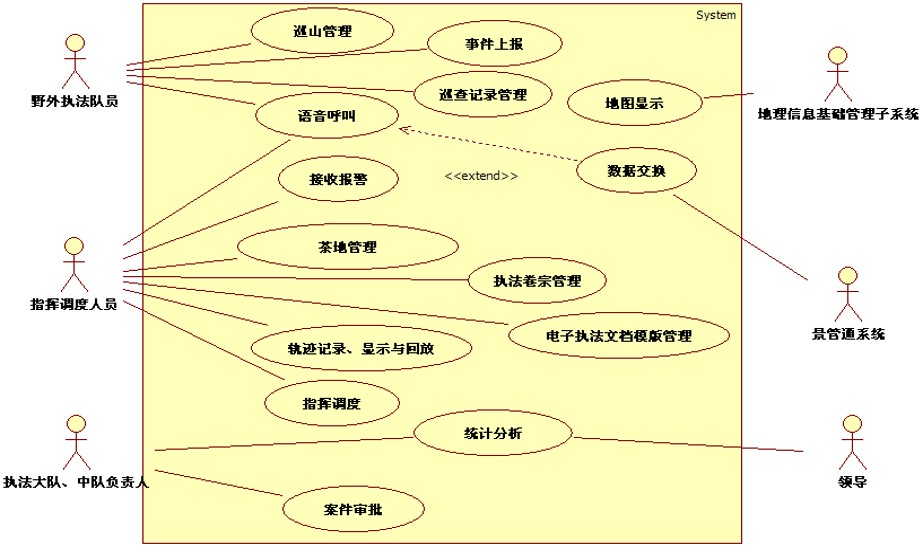
\includegraphics[width=0.65\textwidth]{4_1.jpg}
  \end{center}
\end{figure}
\textbf{执行者}(actor):
\begin{itemize}
  \item 是指用户在系统中所扮演的角色。其图形化的表示是一个小人。
  \item 不带箭头的线段将执行者与用例连接到一起,表示两者之间交换信息,称之为通信联系。
  \item 单个执行者可与多个用例联系;反过来,一个用例可与多个执行者联系。
  \item 执行者可以不是人类用户。
\end{itemize}
\begin{figure}[H]
  \begin{center}
    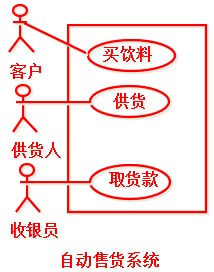
\includegraphics[width=0.25\textwidth]{4_2.jpg}
  \end{center}
\end{figure}
\textbf{用例}:一个用例是用户与系统之间的一次典型交互,代表了将要开发的系统的一项功能。
如:顾客通过B2C电子商务系统下订单。
用例具有以下特点:
\begin{itemize}
  \item 用例捕获某些用户可见的需求,实现一个具体的用户目标。
  \item 用例由执行者激活,并提供确切的结果给执行者。
  \item 用例可大可小,但它必须是对一个具体的用户目标的完整描述。
\end{itemize}
\textbf{用例间的联系}
\begin{itemize}
  \item <<generalization>>表示用例间的继承关系。
  \item <<Extend>>通过向被扩展的用例添加动作来扩展用例。
  \item <<include>>表示一个用例的行为包含了另一个用例的行为。
\end{itemize}
\textbf{包括关系和扩展关系的联系和差别}\\
\textbf{联系}:都是从现有的用例中抽取出公共的那部分信息,作为一个单独的用例。然后通后过不同的方法来重用这个公共的用例,以降低模型维护的工作量。

\textbf{差别}:扩展关系中基本用例的基本流运行时,扩展用例不一定运行,即扩展用例仅仅有在基本用例满足某种条件的时候才会运行。
包括关系中基本用例的基本流运行时。包括用例一定会运行。
\begin{figure}[H]
  \begin{center}
    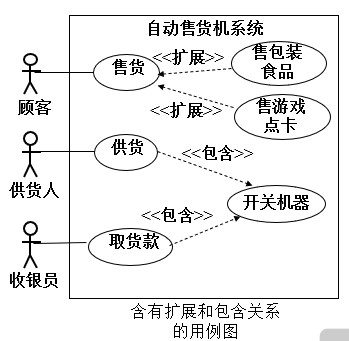
\includegraphics[width=0.25\textwidth]{4_3.jpg}
  \end{center}
\end{figure}
\textbf{用例模型的建立}:建立系统用例模型的过程就是对系统进行功能需求分析的过程。
\begin{enumerate}
  \item 定义系统: 确定系统范围,分析系统功能.
  \item 确定执行者和用例:执行者通常是使用系统功能的外部用户或系统。
    用例是一个子系统或系统的一个独立、完整功能。
  \item 描述执行者和用例关系:各模型元素之间有:关联、泛化、扩展及包含等关系。
  \item 确认模型:确认用例模型与用户需求的一致性,通常由用户与开发者共同完成。
\end{enumerate}
\textbf{获取执行者}:获取用例首先要找出系统的执行者。
可通过用户回答一些问题的答案来识别执行者。以下问题可供参考:
\begin{itemize}
  \item 谁使用系统的主要功能(主要使用者)。
  \item 谁需要系统支持他们的日常工作。
  \item 谁来维护、管理使系统正常工作(辅助使用者)。
  \item 系统需要操纵哪些硬件。
  \item 系统需要与哪些其它系统交互,包含其它计算机系统和其它应用程序。
  \item 对系统产生的结果感兴趣的人或事物。
\end{itemize}
\textbf{获取用例}:一旦获取了执行者,就可以对每个执行者提出问题以获取用例。
\begin{itemize}
  \item 执行者要求系统提供哪些功能(执行者需要做什么)?
  \item 执行者需要读、产生、删除、修改或存储的信息有哪些?
  \item 必须提醒执行者的系统事件有哪些?或者执行者必须提醒系统的事件有哪些?
\end{itemize}
还有一些不针对具体执行者问题(即针对整个系统的问题):
\begin{itemize}
  \item 系统需要何种输入输出?输入从何处来?输出到何处?
  \item 当前运行系统的主要问题?
\end{itemize}
\textbf{角色描述模板}:角色名,角色职责,角色职责识别(使用系统主要功能,对系统运行结果感兴趣).

\textbf{用例描述模板}:用例名,执行者,目标,功能描述,其他非功能需求(可靠,实时),主要步骤,相关用例,
相关信息(优先级,性能,执行频率).
\end{document}
